% Options for packages loaded elsewhere
\PassOptionsToPackage{unicode}{hyperref}
\PassOptionsToPackage{hyphens}{url}
\PassOptionsToPackage{dvipsnames,svgnames,x11names}{xcolor}
%
\documentclass[
  letterpaper,
  DIV=11,
  numbers=noendperiod]{scrartcl}

\usepackage{amsmath,amssymb}
\usepackage{iftex}
\ifPDFTeX
  \usepackage[T1]{fontenc}
  \usepackage[utf8]{inputenc}
  \usepackage{textcomp} % provide euro and other symbols
\else % if luatex or xetex
  \usepackage{unicode-math}
  \defaultfontfeatures{Scale=MatchLowercase}
  \defaultfontfeatures[\rmfamily]{Ligatures=TeX,Scale=1}
\fi
\usepackage{lmodern}
\ifPDFTeX\else  
    % xetex/luatex font selection
\fi
% Use upquote if available, for straight quotes in verbatim environments
\IfFileExists{upquote.sty}{\usepackage{upquote}}{}
\IfFileExists{microtype.sty}{% use microtype if available
  \usepackage[]{microtype}
  \UseMicrotypeSet[protrusion]{basicmath} % disable protrusion for tt fonts
}{}
\makeatletter
\@ifundefined{KOMAClassName}{% if non-KOMA class
  \IfFileExists{parskip.sty}{%
    \usepackage{parskip}
  }{% else
    \setlength{\parindent}{0pt}
    \setlength{\parskip}{6pt plus 2pt minus 1pt}}
}{% if KOMA class
  \KOMAoptions{parskip=half}}
\makeatother
\usepackage{xcolor}
\setlength{\emergencystretch}{3em} % prevent overfull lines
\setcounter{secnumdepth}{-\maxdimen} % remove section numbering
% Make \paragraph and \subparagraph free-standing
\ifx\paragraph\undefined\else
  \let\oldparagraph\paragraph
  \renewcommand{\paragraph}[1]{\oldparagraph{#1}\mbox{}}
\fi
\ifx\subparagraph\undefined\else
  \let\oldsubparagraph\subparagraph
  \renewcommand{\subparagraph}[1]{\oldsubparagraph{#1}\mbox{}}
\fi


\providecommand{\tightlist}{%
  \setlength{\itemsep}{0pt}\setlength{\parskip}{0pt}}\usepackage{longtable,booktabs,array}
\usepackage{calc} % for calculating minipage widths
% Correct order of tables after \paragraph or \subparagraph
\usepackage{etoolbox}
\makeatletter
\patchcmd\longtable{\par}{\if@noskipsec\mbox{}\fi\par}{}{}
\makeatother
% Allow footnotes in longtable head/foot
\IfFileExists{footnotehyper.sty}{\usepackage{footnotehyper}}{\usepackage{footnote}}
\makesavenoteenv{longtable}
\usepackage{graphicx}
\makeatletter
\def\maxwidth{\ifdim\Gin@nat@width>\linewidth\linewidth\else\Gin@nat@width\fi}
\def\maxheight{\ifdim\Gin@nat@height>\textheight\textheight\else\Gin@nat@height\fi}
\makeatother
% Scale images if necessary, so that they will not overflow the page
% margins by default, and it is still possible to overwrite the defaults
% using explicit options in \includegraphics[width, height, ...]{}
\setkeys{Gin}{width=\maxwidth,height=\maxheight,keepaspectratio}
% Set default figure placement to htbp
\makeatletter
\def\fps@figure{htbp}
\makeatother

\KOMAoption{captions}{tableheading}
\makeatletter
\@ifpackageloaded{caption}{}{\usepackage{caption}}
\AtBeginDocument{%
\ifdefined\contentsname
  \renewcommand*\contentsname{Table of contents}
\else
  \newcommand\contentsname{Table of contents}
\fi
\ifdefined\listfigurename
  \renewcommand*\listfigurename{List of Figures}
\else
  \newcommand\listfigurename{List of Figures}
\fi
\ifdefined\listtablename
  \renewcommand*\listtablename{List of Tables}
\else
  \newcommand\listtablename{List of Tables}
\fi
\ifdefined\figurename
  \renewcommand*\figurename{Figure}
\else
  \newcommand\figurename{Figure}
\fi
\ifdefined\tablename
  \renewcommand*\tablename{Table}
\else
  \newcommand\tablename{Table}
\fi
}
\@ifpackageloaded{float}{}{\usepackage{float}}
\floatstyle{ruled}
\@ifundefined{c@chapter}{\newfloat{codelisting}{h}{lop}}{\newfloat{codelisting}{h}{lop}[chapter]}
\floatname{codelisting}{Listing}
\newcommand*\listoflistings{\listof{codelisting}{List of Listings}}
\makeatother
\makeatletter
\makeatother
\makeatletter
\@ifpackageloaded{caption}{}{\usepackage{caption}}
\@ifpackageloaded{subcaption}{}{\usepackage{subcaption}}
\makeatother
\ifLuaTeX
  \usepackage{selnolig}  % disable illegal ligatures
\fi
\usepackage{bookmark}

\IfFileExists{xurl.sty}{\usepackage{xurl}}{} % add URL line breaks if available
\urlstyle{same} % disable monospaced font for URLs
\hypersetup{
  pdftitle={Admission Evaluation Criteria Analysis},
  colorlinks=true,
  linkcolor={blue},
  filecolor={Maroon},
  citecolor={Blue},
  urlcolor={Blue},
  pdfcreator={LaTeX via pandoc}}

\title{Admission Evaluation Criteria Analysis}
\usepackage{etoolbox}
\makeatletter
\providecommand{\subtitle}[1]{% add subtitle to \maketitle
  \apptocmd{\@title}{\par {\large #1 \par}}{}{}
}
\makeatother
\subtitle{DSAN 5900: Digital Storytelling}
\author{Bella Shi \and Samantha Moon \and Lianghui Yi}
\date{}

\begin{document}
\maketitle

\section{Introduction}\label{introduction}

This report provides an analysis of the admissions data to identify key
factors influencing admissions decisions. The goal is to generate
actionable insights for institutional leadership to support strategic
decision-making.

\subsection{Objectives}\label{objectives}

\begin{itemize}
\tightlist
\item
  Understand the distribution of admissions decisions across states.
\item
  Analyze the impact of GPA, test scores, work experience, and volunteer
  levels on admissions.
\item
  Provide actionable recommendations based on data-driven insights.
\end{itemize}

\begin{longtable}[]{@{}
  >{\raggedright\arraybackslash}p{(\columnwidth - 14\tabcolsep) * \real{0.1154}}
  >{\raggedright\arraybackslash}p{(\columnwidth - 14\tabcolsep) * \real{0.1410}}
  >{\raggedleft\arraybackslash}p{(\columnwidth - 14\tabcolsep) * \real{0.0641}}
  >{\raggedleft\arraybackslash}p{(\columnwidth - 14\tabcolsep) * \real{0.1026}}
  >{\raggedleft\arraybackslash}p{(\columnwidth - 14\tabcolsep) * \real{0.1282}}
  >{\raggedleft\arraybackslash}p{(\columnwidth - 14\tabcolsep) * \real{0.1667}}
  >{\raggedleft\arraybackslash}p{(\columnwidth - 14\tabcolsep) * \real{0.0897}}
  >{\raggedleft\arraybackslash}p{(\columnwidth - 14\tabcolsep) * \real{0.1923}}@{}}
\toprule\noalign{}
\begin{minipage}[b]{\linewidth}\raggedright
Decision
\end{minipage} & \begin{minipage}[b]{\linewidth}\raggedright
State
\end{minipage} & \begin{minipage}[b]{\linewidth}\raggedleft
GPA
\end{minipage} & \begin{minipage}[b]{\linewidth}\raggedleft
WorkExp
\end{minipage} & \begin{minipage}[b]{\linewidth}\raggedleft
TestScore
\end{minipage} & \begin{minipage}[b]{\linewidth}\raggedleft
WritingScore
\end{minipage} & \begin{minipage}[b]{\linewidth}\raggedleft
Gender
\end{minipage} & \begin{minipage}[b]{\linewidth}\raggedleft
VolunteerLevel
\end{minipage} \\
\midrule\noalign{}
\endhead
\bottomrule\noalign{}
\endlastfoot
Admit & California & 3.90 & 6.7 & 962 & 100 & 1 & 0 \\
Admit & Florida & 3.80 & 1.4 & 969 & 97 & 1 & 4 \\
Banana & California & 3.80 & 2.3 & 970 & 98 & 0 & 5 \\
Admit & Colorado & 3.60 & 0.9 & 969 & 97 & 0 & 2 \\
Admit & Colorado & 3.92 & 1.2 & 969 & 95 & -1 & 3 \\
NA & California & 3.80 & 1.2 & NA & 95 & 0 & 4 \\
\end{longtable}

\textsubscript{Source:
\href{https://verkyyi.github.io/5900-hw1/index.qmd.html}{Article
Notebook}}

\begin{verbatim}
   Decision            State                GPA           WorkExp      
 Length:88          Length:88          Min.   :2.340   Min.   :  0.00  
 Class :character   Class :character   1st Qu.:3.415   1st Qu.:  1.20  
 Mode  :character   Mode  :character   Median :3.550   Median :  1.55  
                                       Mean   :3.540   Mean   :  3.21  
                                       3rd Qu.:3.745   3rd Qu.:  2.70  
                                       Max.   :6.000   Max.   :100.00  
                                       NA's   :1                       
   TestScore      WritingScore       Gender        VolunteerLevel
 Min.   :751.0   Min.   :  1.0   Min.   :-1.0000   Min.   :0.0   
 1st Qu.:779.0   1st Qu.: 77.0   1st Qu.: 0.0000   1st Qu.:1.0   
 Median :869.0   Median : 85.0   Median : 1.0000   Median :2.0   
 Mean   :875.7   Mean   : 82.6   Mean   : 0.5349   Mean   :2.5   
 3rd Qu.:966.0   3rd Qu.: 93.0   3rd Qu.: 1.0000   3rd Qu.:4.0   
 Max.   :970.0   Max.   :100.0   Max.   : 1.0000   Max.   :5.0   
 NA's   :1                       NA's   :2                       
\end{verbatim}

\textsubscript{Source:
\href{https://verkyyi.github.io/5900-hw1/index.qmd.html}{Article
Notebook}}

\subsection{Data Cleaning}\label{data-cleaning}

\begin{verbatim}
   Decision            State                GPA           WorkExp       
 Length:82          Length:82          Min.   :2.340   Min.   :  0.000  
 Class :character   Class :character   1st Qu.:3.402   1st Qu.:  1.200  
 Mode  :character   Mode  :character   Median :3.545   Median :  1.550  
                                       Mean   :3.528   Mean   :  3.324  
                                       3rd Qu.:3.700   3rd Qu.:  2.700  
                                       Max.   :6.000   Max.   :100.000  
   TestScore      WritingScore        Gender      VolunteerLevel 
 Min.   :751.0   Min.   :  1.00   Min.   :0.000   Min.   :0.000  
 1st Qu.:769.0   1st Qu.: 77.00   1st Qu.:0.000   1st Qu.:1.000  
 Median :868.0   Median : 84.00   Median :1.000   Median :2.000  
 Mean   :871.2   Mean   : 81.84   Mean   :0.561   Mean   :2.427  
 3rd Qu.:965.8   3rd Qu.: 92.50   3rd Qu.:1.000   3rd Qu.:4.000  
 Max.   :969.0   Max.   :100.00   Max.   :1.000   Max.   :5.000  
\end{verbatim}

\textsubscript{Source:
\href{https://verkyyi.github.io/5900-hw1/index.qmd.html}{Article
Notebook}}

\subsection{Visualizations and
Analysis}\label{visualizations-and-analysis}

\subsubsection{1. Admission Rates by
State}\label{admission-rates-by-state}

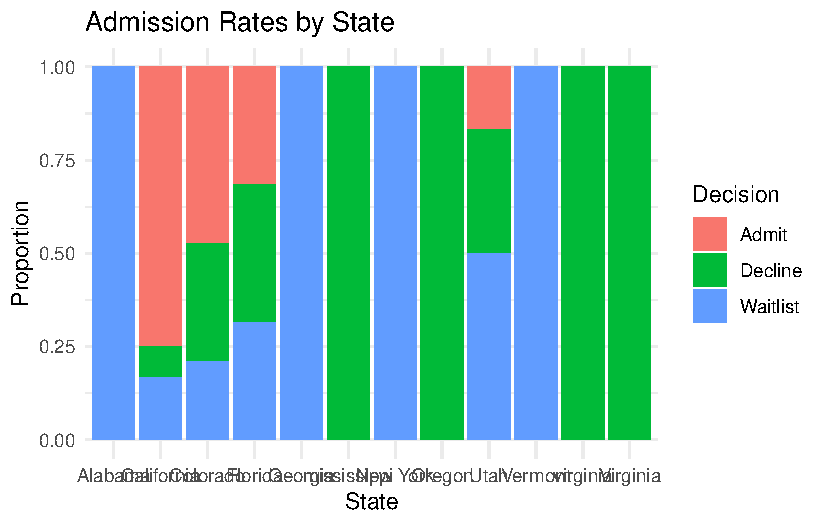
\includegraphics{index_files/figure-pdf/admission-rates-by-state-1.pdf}

\textsubscript{Source:
\href{https://verkyyi.github.io/5900-hw1/index.qmd.html}{Article
Notebook}}

\textbf{Analysis:} The visualization highlights which states have higher
or lower admission rates. States with consistently low acceptance rates
may need targeted recruitment strategies or support programs.

\subsubsection{2. GPA and Test Scores for Admitted vs.~Rejected
Students}\label{gpa-and-test-scores-for-admitted-vs.-rejected-students}

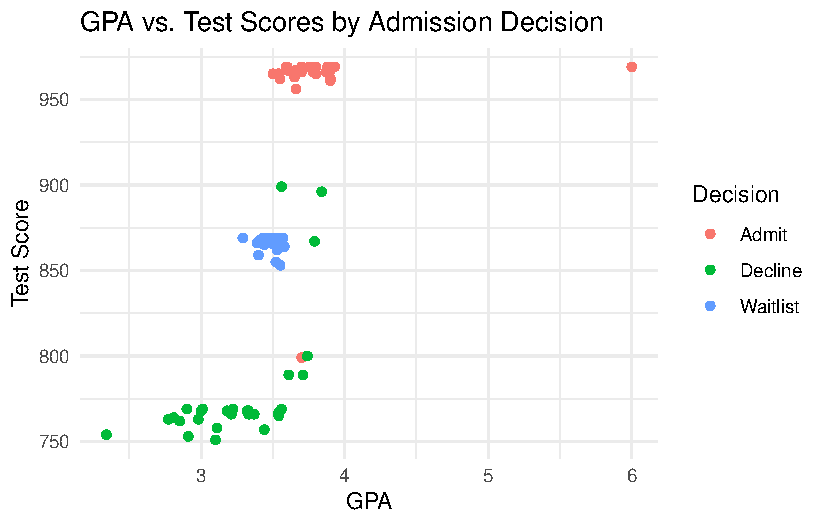
\includegraphics{index_files/figure-pdf/gpa-testscore-distribution-1.pdf}

\textsubscript{Source:
\href{https://verkyyi.github.io/5900-hw1/index.qmd.html}{Article
Notebook}}

\textbf{Analysis:} This scatter plot reveals how GPA and test scores
correlate with admissions decisions. Students with higher GPAs and test
scores generally have a higher chance of being admitted.

\subsubsection{3. Correlation Heatmap}\label{correlation-heatmap}

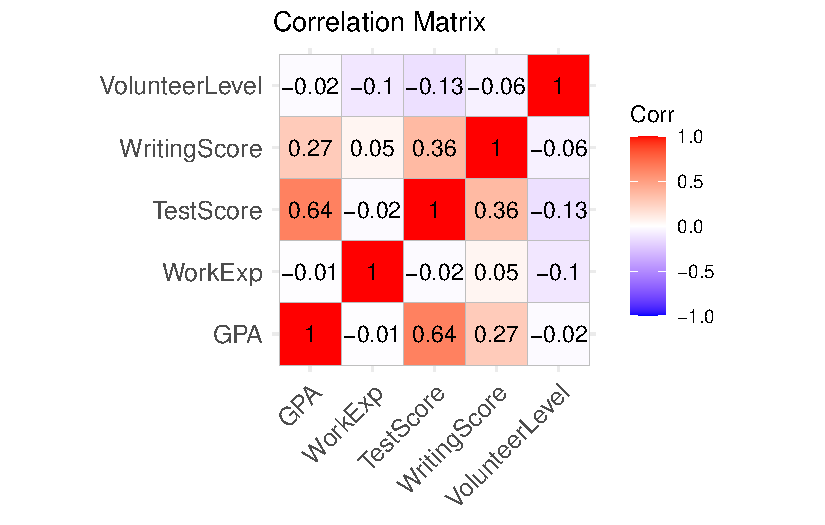
\includegraphics{index_files/figure-pdf/correlation-heatmap-1.pdf}

\textsubscript{Source:
\href{https://verkyyi.github.io/5900-hw1/index.qmd.html}{Article
Notebook}}

\textbf{Analysis:} The heatmap shows the correlations between
quantitative variables. Strong correlations can help identify which
metrics are most predictive of admissions success.

\subsubsection{4. Grouped boxplot}\label{grouped-boxplot}

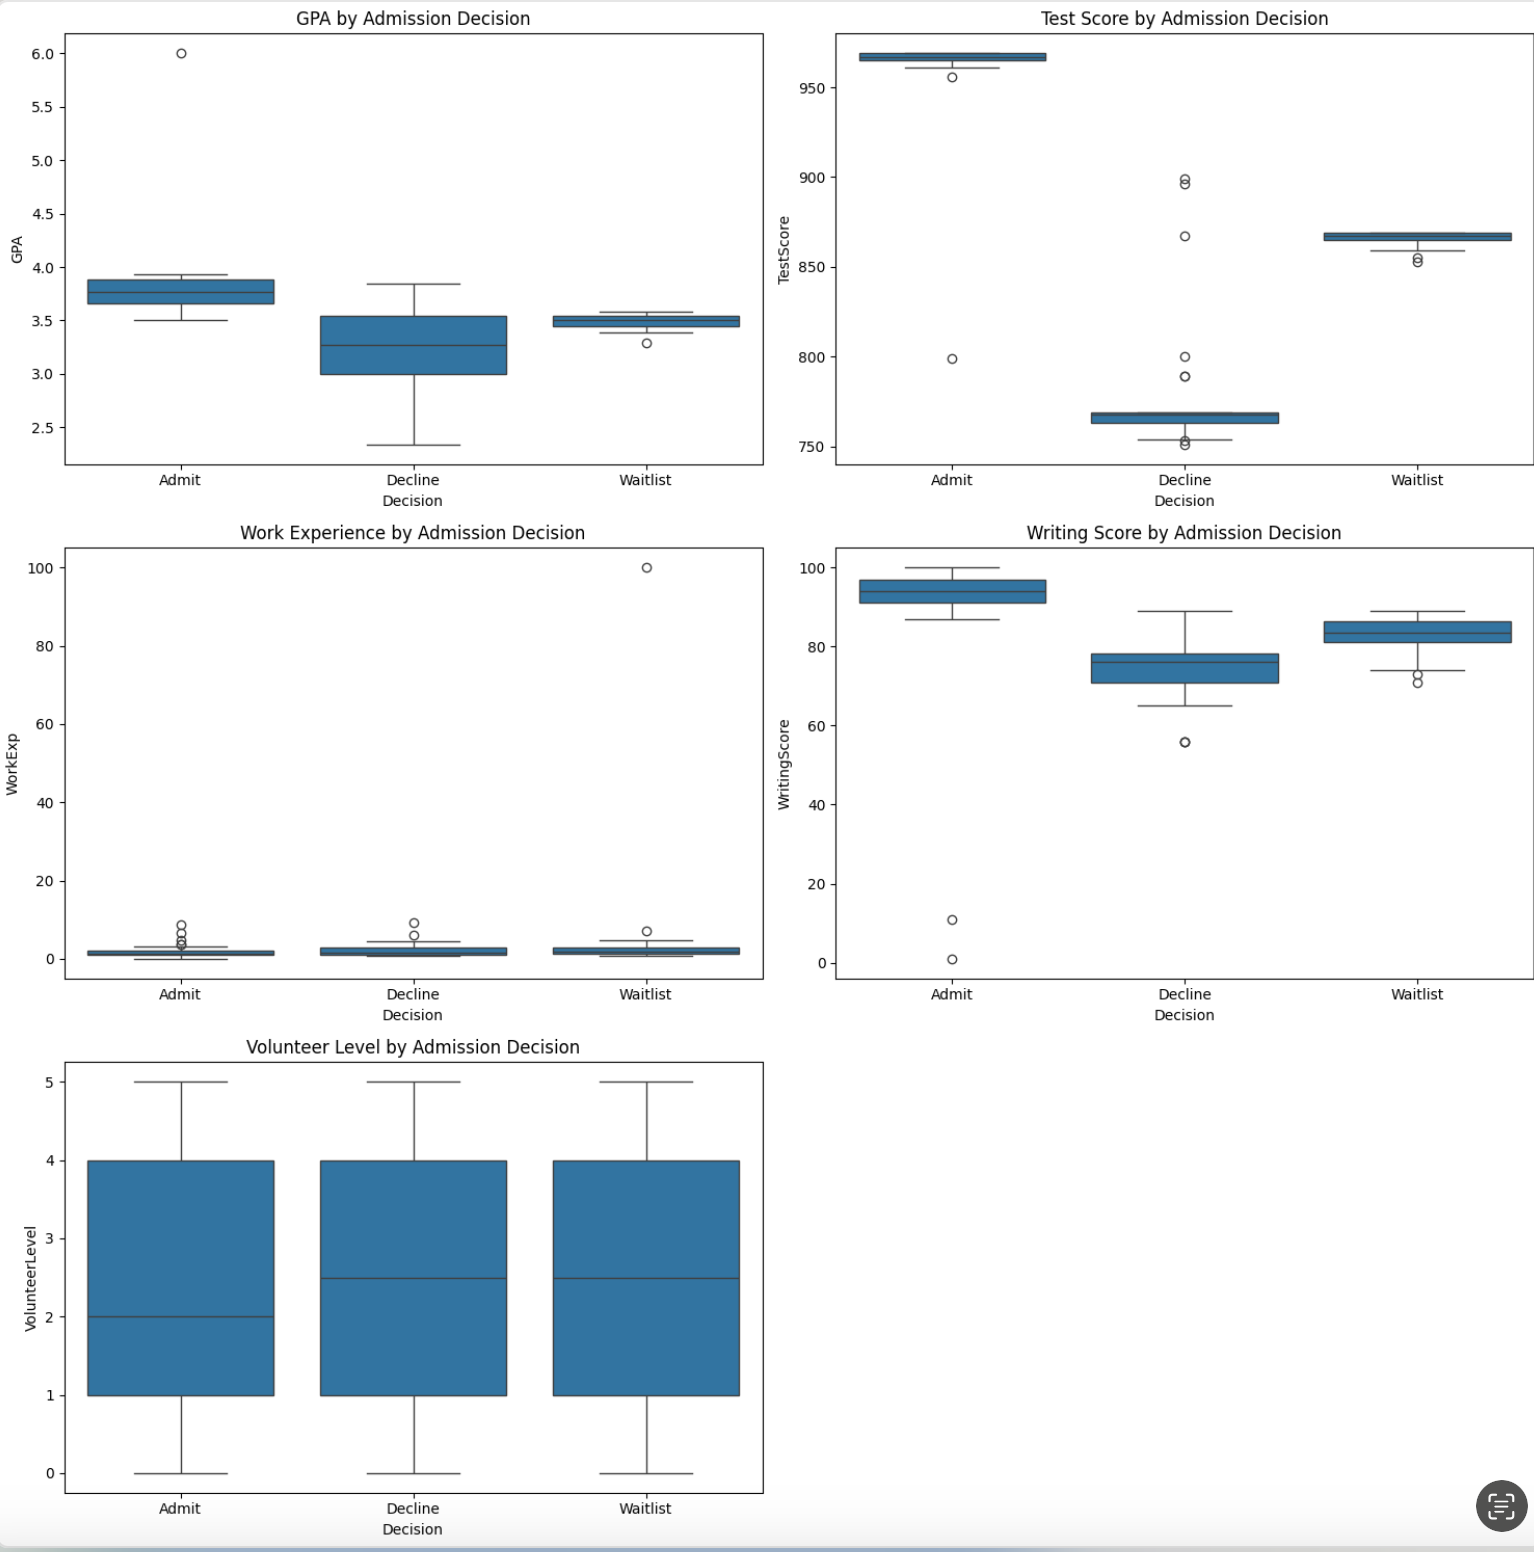
\includegraphics{images/paste-1.png}

\textbf{Analysis:} This grouped boxplot provides insights into the
distribution of admissions criteria.

Key observations include:

\begin{itemize}
\item
  GPA/ and Admission Relationship: The visualization confirms that
  applicants with a GPA above a certain threshold (e.g., 3.5) have a
  significantly higher chance of admission.
\item
  Test score and Admission Relationship: A sharp increase in acceptance
  rates is observed in the 900-1000 test score range
\item
  High writing scores (90-100) improve chances for getting admission
\item
  Volunteer Experience Impact: it appears to have minimal impact on the
  final admission decision
\end{itemize}

\subsection{Conclusion}\label{conclusion}

\subsubsection{GPA Impact}\label{gpa-impact}

\begin{enumerate}
\def\labelenumi{\arabic{enumi}.}
\tightlist
\item
  High GPAs (3.0-3.5 and 3.5-4.0) have significantly higher acceptance
  rates, with the 3.5-4.0 range being the strongest predictor of
  acceptance.
\item
  Suggests that academic performance is a critical factor in the
  admission process.
\end{enumerate}

\subsubsection{Test Scores}\label{test-scores}

\begin{enumerate}
\def\labelenumi{\arabic{enumi}.}
\tightlist
\item
  A sharp increase in acceptance rates is observed in the 900-1000 test
  score range.
\item
  Emphasizes the importance of standardized testing in the selection
  process.
\end{enumerate}

\subsubsection{Writing Scores}\label{writing-scores}

\begin{enumerate}
\def\labelenumi{\arabic{enumi}.}
\tightlist
\item
  High writing scores (90-100) improve acceptance chances, but the
  acceptance rate is still significantly lower compared to other
  metrics.
\item
  Indicates writing score might be a secondary factor or less emphasized
  compared to GPA and test scores.
\end{enumerate}

\subsubsection{Work Experience}\label{work-experience}

\begin{enumerate}
\def\labelenumi{\arabic{enumi}.}
\tightlist
\item
  Applicants with less work experience (0-20 years) show higher
  acceptance rates.
\item
  This might indicate a preference for younger applicants or those
  earlier in their career paths, possibly aligning with program goals
  targeting recent graduates or early-career professionals.
\end{enumerate}

\subsubsection{Volunteer Level}\label{volunteer-level}

\begin{enumerate}
\def\labelenumi{\arabic{enumi}.}
\tightlist
\item
  Volunteer levels do not show a strong correlation with acceptance
  rates, suggesting this might not be a significant criterion in the
  current evaluation process.
\end{enumerate}

\subsubsection{Applicant's Stat}\label{applicants-stat}

\begin{enumerate}
\def\labelenumi{\arabic{enumi}.}
\tightlist
\item
  There is a notable geographical impact on acceptance rates, with
  California having the highest acceptance rate.
\item
  States like Alabama, Vermont, and Virginia also show strong acceptance
  metrics, while other states may need more targeted outreach or
  support.
\end{enumerate}

\subsection{Suggestions for Future Admission
Evaluations:}\label{suggestions-for-future-admission-evaluations}

\begin{enumerate}
\def\labelenumi{\arabic{enumi}.}
\item
  Enhance GPA Weighting: • Maintain or increase the emphasis on academic
  performance, particularly for applicants with GPAs above 3.0. •
  Consider adding additional weight to applicants from rigorous academic
  institutions or challenging coursework.
\item
  Reevaluate Work Experience Criteria: • Consider whether the preference
  for less work experience aligns with program goals. If diversity in
  professional backgrounds is desired, adjust admission strategies
  accordingly.
\item
  Writing Skills Assessment: • If writing is a critical skill for
  success in the program, enhance the evaluation of writing samples or
  essays. Alternatively, if writing scores are not as crucial,
  streamline this criterion to focus on higher-impact factors.
\item
  Volunteer Experience Consideration: • Since volunteer experience does
  not show a strong influence on acceptance rates, consider
  de-emphasizing this criterion unless community service is a core value
  of the institution.
\end{enumerate}

\subsection{Marketing Campaign
Suggestions:}\label{marketing-campaign-suggestions}

\begin{enumerate}
\def\labelenumi{\arabic{enumi}.}
\tightlist
\item
  Target High-Performing Students

  \begin{itemize}
  \tightlist
  \item
    Focus outreach efforts on students with high GPAs and strong
    standardized test scores.
  \item
    Collaborate with high schools, undergraduate institutions, and
    tutoring centers to attract these candidates.
  \end{itemize}
\item
  Regional Campaigns

  \begin{itemize}
  \tightlist
  \item
    Implement targeted marketing in high-acceptance regions such as
    California, Virginia, and Vermont.
  \item
    For states with lower acceptance rates, explore potential barriers
    (e.g., awareness, application support) and address them through
    localized campaigns.
  \end{itemize}
\end{enumerate}

\subsection{Overall Strategy}\label{overall-strategy}

\begin{enumerate}
\def\labelenumi{\arabic{enumi}.}
\tightlist
\item
  By focusing on academic excellence and regional strengths, while
  adjusting evaluation criteria to align with institutional priorities,
  the admissions team can enhance both the quality and diversity of
  incoming students.
\item
  Simultaneously, targeted and data-driven marketing efforts will ensure
  that the institution attracts well-qualified applicants and improves
  overall admission outcomes.
\end{enumerate}



\end{document}
